\documentclass[11pt]{article}

\usepackage[margin=1in]{geometry}
\usepackage{booktabs}
\usepackage{fontspec}
\usepackage{float}
\usepackage{graphicx}
\usepackage[hidelinks]{hyperref}
\usepackage{longtable}
\usepackage{microtype}
\usepackage{pdflscape}
\usepackage{placeins}
\usepackage{setspace}
\usepackage{tabularx}
\usepackage{threeparttable}
\usepackage[backend=biber,style=authoryear,maxcitenames=2,maxbibnames=20]{biblatex}

\setlength{\emergencystretch}{1em}

\addbibresource{../lit/references.bib}
\newcommand{\FFROriginalGain}{70.9}
\newcommand{\FFROriginalLoss}{41.1}
\newcommand{\FFROriginalEffect}{29.8}
\newcommand{\FFROriginalLow}{19.0}
\newcommand{\FFROriginalHigh}{40.6}
\newcommand{\FFROriginalN}{299}
\newcommand{\LuthOriginalGain}{61.6}
\newcommand{\LuthOriginalLoss}{36.4}
\newcommand{\LuthOriginalEffect}{25.2}
\newcommand{\LuthOriginalLow}{12.5}
\newcommand{\LuthOriginalHigh}{37.8}
\newcommand{\LuthOriginalN}{232}
\newcommand{\LuthMinimumEffect}{7.8}
\newcommand{\LuthMaximumEffect}{39.2}
\newcommand{\FFRMinimumEffect}{26.6}
\newcommand{\FFRMaximumEffect}{38.5}
\newcommand{\FFRArmOriginalEffect}{29.8}
\newcommand{\FFRArmOriginalLow}{19.0}
\newcommand{\FFRArmOriginalHigh}{40.6}
\newcommand{\FFRArmRiskyFlipEffect}{26.6}
\newcommand{\FFRArmRiskyFlipLow}{15.7}
\newcommand{\FFRArmRiskyFlipHigh}{37.4}
\newcommand{\FFRArmRewordingEffect}{38.5}
\newcommand{\FFRArmRewordingLow}{27.9}
\newcommand{\FFRArmRewordingHigh}{49.1}
\newcommand{\LuthArmOriginalEffect}{25.2}
\newcommand{\LuthArmOriginalLow}{12.5}
\newcommand{\LuthArmOriginalHigh}{37.8}
\newcommand{\LuthArmLowerEffect}{16.9}
\newcommand{\LuthArmLowerLow}{3.5}
\newcommand{\LuthArmLowerHigh}{30.2}
\newcommand{\LuthArmUpperEffect}{33.7}
\newcommand{\LuthArmUpperLow}{20.6}
\newcommand{\LuthArmUpperHigh}{46.7}
\newcommand{\LuthArmResponseOrderEffect}{27.6}
\newcommand{\LuthArmResponseOrderLow}{15.1}
\newcommand{\LuthArmResponseOrderHigh}{40.2}
\newcommand{\LuthArmBalancedEffect}{17.9}
\newcommand{\LuthArmBalancedLow}{4.9}
\newcommand{\LuthArmBalancedHigh}{30.9}
\newcommand{\LuthArmBalancedReversedEffect}{7.8}
\newcommand{\LuthArmBalancedReversedLow}{-5.2}
\newcommand{\LuthArmBalancedReversedHigh}{20.8}
\newcommand{\LuthArmRiskyFlipEffect}{27.2}
\newcommand{\LuthArmRiskyFlipLow}{13.9}
\newcommand{\LuthArmRiskyFlipHigh}{40.5}
\newcommand{\LuthArmRiskyResponseEffect}{39.2}
\newcommand{\LuthArmRiskyResponseLow}{28.0}
\newcommand{\LuthArmRiskyResponseHigh}{50.5}

\newcommand{\FFRHeterogeneityF}{1.29}
\newcommand{\FFRHeterogeneityP}{0.275}
\newcommand{\LuthHeterogeneityF}{2.51}
\newcommand{\LuthHeterogeneityP}{0.014}

\newcommand{\ModeratorMinimumHolmP}{0.008}
\newcommand{\EducationMetaK}{5}
\newcommand{\EducationMetaEffect}{4.0}
\newcommand{\EducationMetaLow}{2.7}
\newcommand{\EducationMetaHigh}{5.2}
\newcommand{\EducationMetaP}{0.001}
\newcommand{\EducationMetaISquared}{0.0}
\newcommand{\EducationMetaPredLow}{2.7}
\newcommand{\EducationMetaPredHigh}{5.2}
\newcommand{\ModeratorArchiveInteraction}{3.8}
\newcommand{\ModeratorArchiveLow}{0.8}
\newcommand{\ModeratorArchiveHigh}{6.8}
\newcommand{\ModeratorAllInteraction}{4.0}
\newcommand{\ModeratorAllLow}{1.5}
\newcommand{\ModeratorAllHigh}{6.6}

\newcommand{\ProtzkoN}{4,585}
\newcommand{\ProtzkoOriginalContrast}{32.9}
\newcommand{\ProtzkoOriginalLow}{27.5}
\newcommand{\ProtzkoOriginalHigh}{38.3}
\newcommand{\ProtzkoOriginalMin}{31.4}
\newcommand{\ProtzkoOriginalMax}{34.1}
\newcommand{\ProtzkoFlipContrast}{31.3}
\newcommand{\ProtzkoFlipLow}{25.8}
\newcommand{\ProtzkoFlipHigh}{36.8}
\newcommand{\ProtzkoFlipMin}{23.1}
\newcommand{\ProtzkoFlipMax}{38.9}
\newcommand{\ProtzkoBalancedContrast}{12.6}
\newcommand{\ProtzkoBalancedLow}{6.8}
\newcommand{\ProtzkoBalancedHigh}{18.4}
\newcommand{\ProtzkoBalancedMin}{7.6}
\newcommand{\ProtzkoBalancedMax}{20.6}
\newcommand{\ProtzkoBalancedFlipContrast}{15.1}
\newcommand{\ProtzkoBalancedFlipLow}{9.4}
\newcommand{\ProtzkoBalancedFlipHigh}{20.8}
\newcommand{\ProtzkoBalancedFlipMin}{3.6}
\newcommand{\ProtzkoBalancedFlipMax}{37.4}
\newcommand{\ProtzkoExplicitInteraction}{-20.4}
\newcommand{\ProtzkoExplicitLow}{-28.3}
\newcommand{\ProtzkoExplicitHigh}{-12.5}
\newcommand{\ProtzkoExplicitAttenuation}{20.4}
\newcommand{\ProtzkoExplicitAttenuationLow}{12.5}
\newcommand{\ProtzkoExplicitAttenuationHigh}{28.3}
\newcommand{\ProtzkoExplicitP}{<.001}
\newcommand{\ProtzkoFlipInteraction}{-1.7}
\newcommand{\ProtzkoFlipP}{0.659}
\newcommand{\ProtzkoThreeWay}{4.4}
\newcommand{\ProtzkoThreeWayP}{0.446}

\newcommand{\OpenEndedN}{1,752}
\newcommand{\OpenEndedCertaintyGain}{23.7}
\newcommand{\OpenEndedCertaintyLoss}{26.7}
\newcommand{\OpenEndedCertaintyDiff}{2.8}
\newcommand{\OpenEndedChanceGain}{33.3}
\newcommand{\OpenEndedChanceLoss}{31.1}
\newcommand{\OpenEndedChanceDiff}{-2.0}

\newcommand{\ArchiveMetaK}{23}
\newcommand{\ArchiveMetaN}{7,249}
\newcommand{\ArchiveMetaEffect}{24.7}
\newcommand{\ArchiveMetaLow}{19.7}
\newcommand{\ArchiveMetaHigh}{29.7}
\newcommand{\ArchiveMetaPredLow}{2.7}
\newcommand{\ArchiveMetaPredHigh}{46.6}
\newcommand{\ArchiveMetaISquared}{78.5}
\newcommand{\ArchiveMetaTau}{0.103}

\newcommand{\FlipChangeEffect}{-1.3}
\newcommand{\FlipChangeLow}{-7.8}
\newcommand{\FlipChangeHigh}{5.3}
\newcommand{\FlipChangeK}{5}
\newcommand{\BalancedAttenuation}{18.1}
\newcommand{\BalancedAttenuationLow}{5.0}
\newcommand{\BalancedAttenuationHigh}{31.2}
\newcommand{\BalancedFlipAttenuation}{17.5}
\newcommand{\BalancedFlipAttenuationLow}{-30.1}
\newcommand{\BalancedFlipAttenuationHigh}{65.0}
\newcommand{\BalancedChangeEffect}{-18.1}
\newcommand{\BalancedChangeLow}{-31.2}
\newcommand{\BalancedChangeHigh}{-5.0}
\newcommand{\BalancedChangeK}{4}
\newcommand{\BalancedFlipChangeEffect}{-17.5}
\newcommand{\BalancedFlipChangeLow}{-65.0}
\newcommand{\BalancedFlipChangeHigh}{30.1}
\newcommand{\BalancedFlipChangeK}{3}
\newcommand{\BalancedReversedChangeEffect}{-17.3}
\newcommand{\BalancedReversedChangeLow}{-35.3}
\newcommand{\BalancedReversedChangeHigh}{0.7}
\newcommand{\BalancedReversedChangeK}{1}
\newcommand{\ResponseOrderChangeEffect}{2.5}
\newcommand{\ResponseOrderChangeLow}{-15.2}
\newcommand{\ResponseOrderChangeHigh}{20.2}
\newcommand{\ResponseOrderChangeK}{1}
\newcommand{\RiskyResponseChangeEffect}{14.1}
\newcommand{\RiskyResponseChangeLow}{-2.7}
\newcommand{\RiskyResponseChangeHigh}{30.9}
\newcommand{\RiskyResponseChangeK}{1}
\newcommand{\LowerChangeEffect}{-8.3}
\newcommand{\LowerChangeLow}{-26.5}
\newcommand{\LowerChangeHigh}{10.0}
\newcommand{\LowerChangeK}{1}
\newcommand{\UpperChangeEffect}{8.5}
\newcommand{\UpperChangeLow}{-9.5}
\newcommand{\UpperChangeHigh}{26.5}
\newcommand{\UpperChangeK}{1}
\newcommand{\RewordChangeEffect}{8.7}
\newcommand{\RewordChangeLow}{-6.4}
\newcommand{\RewordChangeHigh}{23.8}
\newcommand{\RewordChangeK}{1}


\title{Description Invariance in Risky-Choice Framing:\
Evidence from Five Survey Experiments}
\author{John Protzko \and Gaurav Sood \and Jon A. Krosnick}
\date{Draft: \today}

\begin{document}
\maketitle

\begin{abstract}
Description invariance is a foundational requirement of rational choice: two descriptions of the same prospect should elicit the same preference. The Asian Disease Problem is its canonical violation; in the original demonstration, describing identical outcomes as lives saved rather than lives lost moved the share choosing the certain option by 50 percentage points. Five randomized survey experiments spanning nine years show that the direction of that violation is a stable fact but its size is not. The archive comprises \ArchiveMetaN\ respondents and \ArchiveMetaK\ independent gain-loss contrasts: a national area-probability panel, a volunteer panel that fielded nine versions of the problem, and three factorial experiments that ran an identical instrument, with every deployed treatment documented arm by arm. Every contrast is positive, and the average of \ArchiveMetaEffect\ points (95\% CI \ArchiveMetaLow\ to \ArchiveMetaHigh) is enough to move roughly one respondent in four. The size instead tracks what the descriptions leave unstated. Relative to each survey's original wording, fully stating the certain option removed more than half of the effect (\BalancedAttenuation\ points across the four surveys that fielded it), while reversing the order of the risky option's outcomes left the effect essentially unchanged (\FlipChangeEffect\ points across five surveys). The contrast also grows modestly with education (\EducationMetaEffect\ points per category, exploratory). This pattern is consistent with respondents drawing inferences from incomplete descriptions rather than reacting to gain and loss labels alone. The analysis is a retrospective specification over archival records, and we present it as an audited replication and robustness study.
\end{abstract}

\onehalfspacing

\section{Introduction}

Equivalent gain and loss descriptions of the Asian Disease problem produced a higher certain-choice rate in the gain frame in all 23 valid contrasts from five archival experiments. But the size of that contrast varied with the wording of the options. The paper asks a narrower and more useful question than whether wording matters: which aspects of a risky-choice description preserve the classic direction, and which change its magnitude?

The Asian Disease Problem asks respondents to choose between a certain program and a risky program with the same expected outcome. In the original experiment, 72 percent chose the certain program when outcomes were described as lives saved, while 22 percent chose its equivalent when outcomes were described as lives lost \parencite{tversky1981framing}. The result became a central illustration of risky-choice framing and an application of prospect theory \parencite{kahneman1979prospect,levin1998typology}. It is also a direct failure of description invariance: if two descriptions represent the same prospect, a stable preference should not depend on which description is used \parencite{kahneman1984choices}.

The canonical task leaves open what, exactly, respondents represent. The certain gain says that 200 people will be saved but says nothing about the other 400. The certain loss says that 400 people will die but says nothing about the other 200. Under the intended reading, both descriptions represent 200 survivors and 400 deaths. But the unstated complement may invite different inferences about the people not mentioned. The task also always lists the certain option first and presents the two outcomes of the risky option in one order. Those presentation choices do not confound the randomized frame contrast by themselves. They can matter, though, if their effects interact with the frame or change how respondents construe the alternatives.

This distinction is theoretical as well as methodological. Prospect theory attributes the shift to evaluation relative to a reference point and to different attitudes toward risk in gains and losses \parencite{kahneman1979prospect,tversky1992advances}. Fuzzy-trace theory emphasizes the qualitative contrast between saving some people for sure and risking that none are saved \parencite{reyna1991fuzzy,kuhberger2010task}. Linguistic and communicative accounts distinguish the wording of a descriptor from the outcome it denotes, treat unstated complements as an interpretive problem, or treat a speaker's choice of frame as information \parencite{mandel2001gainloss,mckenzie2003speaker,sher2006information}. Explicated-valence and query-theory accounts instead focus on the valence of the stated components and on the order in which option-favoring reasons come to mind \parencite{tombu2015valence,wall2020query,composto2025query}. A gain-loss difference alone cannot choose among these accounts.

Prior work shows why that restraint matters. Changing causal information or making quantifiers explicit can change the interpretation of incomplete options \parencite{jou1996schemas,mandel2014irrational}. Changing which complements are stated can attenuate, eliminate, or reverse the standard contrast \parencite{kuhberger1995newlook,kuhberger2010task,zhou2021descriptions}. But framing can survive intensive linguistic disambiguation \parencite{chick2016ambiguity}. Recent designs that vary matched and mismatched descriptions find that description valence explains substantial variation while a residual framing effect remains even when options are matched and complete \parencite{dekay2024mismatched,dekay2026complete}. The live theoretical issue is therefore not whether one wording artifact explains the Asian Disease result. It is which description features alter choice and which leave the directional contrast intact.

The broader evidence makes the same point. The directional pattern appears in the original meta-analysis and its reanalysis, a multilaboratory replication, a 49-country study, and recent systematic and meta-analytic reviews \parencite{kuhberger1998meta,klein2014manylabs,steiger2018reappraisal,im2022crossnational,kuhberger2023systematic,ding2025meta}. Yet task domain, probabilities, option descriptions, and procedures contribute to heterogeneity \parencite{kuhberger1999reflection,diederich2018moderators,dekay2022metastudies}. A useful paper should therefore report both the direction of the gain-loss contrast and the task conditions under which its size changes.

We use five archival experiments to do that. Two 2009 experiments, one fielded in a U.S. area-probability online panel and one in a screened volunteer panel, vary response order, the order of outcomes within the risky option, the expected outcome of the certain option, whether the certain option states both outcomes, and the scenario wording. The 199 and 201 wording pairs are especially informative: within each pair, the gain and loss descriptions remain equivalent, while the certain outcome moves one life below or above the gamble's expected outcome. They test local description invariance, not a full value function. Three 2018 factorial experiments independently cross the frame with risky-option order and a balanced certain-option description. The 23 resulting gain-loss contrasts permit feature-specific estimates and an archive-wide synthesis of heterogeneity.

Several of these manipulations recur across surveys: reversing the outcome order within the risky option was fielded in both 2009 surveys and randomized in all three 2018 experiments, and fully stating the certain option was fielded in the volunteer panel and randomized in 2018. We therefore organize the results by manipulation, reporting every estimate of each wording change together, with the surveys as replications. The two vintages still contribute different kinds of estimates. The 2009 variants yield pair-specific framing contrasts that ask whether the classic effect survives a plausible change to a deployed survey question. The 2018 factorial experiments additionally yield interaction terms that estimate how a manipulation changes the contrast. We keep those quantities labeled throughout, and we use the archive-wide meta-analysis only to summarize the distribution of valid gain-loss contrasts, not to manufacture a single universal effect size.

The experiments predate much of the literature that now frames these issues, but the current analysis does not. Earlier scripts and outputs were available before the present specification was written. We therefore treat the study as a retrospective archival analysis, report effect sizes and uncertainty, and avoid confirmatory or priority claims.

\section{Methods}

\subsection{Experimental logic and estimands}

Each study contributes a gain-minus-loss risk difference: the proportion choosing the certain option in the gain frame minus the corresponding proportion in the loss frame. A positive value is the classic framing direction. The key estimand is not a single universal effect size but the change in that risk difference under each wording or representation manipulation.

The 2009 experiments vary the written description while preserving randomized gain-versus-loss assignment within wording pairs. These variants test description invariance and the sensitivity of the contrast to order, completeness, and expected-outcome wording. The 2018 experiments use a factorial design in which frame is crossed with an internal flip of the risky option's outcome order and a factor historically described as a balanced statement of the certain outcomes. Their interaction terms estimate how each manipulation changes the gain-minus-loss contrast. These are tests of description invariance, not estimates of a value function, probability-weighting function, or other structural parameter of prospect theory.

Throughout, an \emph{arm} is a numbered randomized condition; a \emph{wording pair} is a gain-loss pair of arms in a 2009 experiment; a \emph{design cell} is a combination of the two 2018 factors; and a \emph{manipulation family} groups the wording pairs and design cells that implement the same textual change, wherever it was fielded. The family taxonomy is descriptive: it names which deployed treatments alter the same feature of the problem so that their estimates can be read together, and the analysis registry encodes it so that every exhibit uses the same assignment and labels. Reversing the risky option's outcome order appears in all five experiments; fully stating the certain option appears in the volunteer panel and, as the functionally described balanced factor, in all three 2018 experiments.

\subsection{Samples and data provenance}

Stanford University and Abt SRBI built the Face-to-Face Recruited Internet Survey Platform, or FFRISP, with National Science Foundation funding \parencite{ackermann2009ffrisp}. Its target population was English-speaking adult household residents in the 50 states and the District of Columbia. The three-stage area-probability design sampled 50 primary sampling units, 256 segments, and 3,723 addresses. Interviewers screened households and used an automated system to select one adult at random. Of 1,145 selected eligible adults, 1,000 enrolled during 2008.

The recruitment offer described the study, incentives, and participants' rights before consent. All enrollees were offered a Dell Vostro 1000 laptop for the 12-month panel; 57 who already owned a computer and declined another received up to \$500 instead. Abt SRBI paid for high-speed internet for about 260 households and offered quarterly completion incentives. The framing experiment appeared in the twelfth monthly survey in September 2009. The export contains 902 completed records. Four test or nonpanel identifiers were removed, leaving 898 respondents; 887 supplied a valid framing choice. All 898 matched the panel profile, and 896 matched the archived month 12 weight. Appendix Table~\ref{tab:ffrisp-retention} reports retention across all 12 waves.

The Luth volunteer-panel experiment was completed by 2,330 respondents from October 7 through October 14, 2009. A question presented before the experiment asked respondents to select a specified response. The primary analysis includes the 2,017 respondents who complied. Arms 7 and 8 formed a planned gain-loss pair, but the deployed loss-frame stem named Programs C and D while the response options named Programs A and B. We exclude both arms, leaving 1,777 respondents in valid wording pairs. A sensitivity analysis retains all completed respondents while continuing to exclude the defective pair.

The available 2018 archive contains two survey exports labeled Stanford discovery and Stanford replication and one labeled UCSB replication. They contain 1,647, 1,442, and 1,500 respondents, respectively. Four Stanford respondents lack a valid first choice, leaving \ProtzkoN\ observations. The Stanford exports record two frame questions per respondent; we use only the first, matching the received anonymous combined file and avoiding carryover from a prior frame. The UCSB export contributes one choice per respondent. The original questionnaire, sampling documentation, and November 2019 manuscript are not present in the archive, so institutional labels identify the archived studies but do not establish their sampling frames.

\subsection{Design and measures}

Within each wording pair, odd-numbered conditions used a gain frame and even-numbered conditions used a loss frame. Each respondent saw one condition. The outcome equals one for choosing the certain option and zero for choosing the risky option. Response coding accounts for conditions in which the risky option appeared first.

FFRISP included three wording pairs: the original wording, a reversal of the outcome order within the risky option, and an expanded scenario involving two drugs. Luth included the original plus eight planned variants. Two variants changed the certain outcome to 199 saved and 401 lost, or to 201 saved and 399 lost. Within each variant, the gain and loss descriptions specify the same sure outcome and the risky option remains unchanged. The 199, 200, and 201 pairs therefore provide three local tests of description invariance while moving the sure outcome around the gamble's expected outcome. Other variants reversed response order, stated both parts of the certain outcome, reversed the order of those parts, reversed the order of outcomes within the risky option, or combined risky-outcome and response-order reversals. The ninth planned pair used natural-frequency language but is excluded because of the instrument defect.

Education was harmonized into four ordered categories. The Luth political survey also included five factual questions about national institutions and officeholders. We score the proportion correct only for respondents who completed that survey. This battery measures political knowledge, not intelligence or general cognitive ability.

The 2018 exports record three binary factors: gain versus loss frame, original versus internally flipped presentation, and whether the certain option was balanced by stating both outcomes. The complete fielded wording is unavailable, so we describe the balanced factor functionally rather than quote its text. The Stanford exports also carry the questionnaire's block-assignment labels, which name each arm and its frame order; the build verifies that these labels agree with the recorded factor coding for every respondent, and the UCSB export's precomputed interaction columns pass the analogous check. Source code $-99$ is treated as item nonresponse. The received four-variable combined file is not used as an analytical source because it adds one blank row and changes one source-missing first choice to zero.

\subsection{Estimands and inference}

For each wording pair, the estimand is the gain-frame proportion choosing the certain option minus the corresponding loss-frame proportion. We estimate this difference with a linear probability model and HC2 standard errors. The point estimate is exactly the raw difference in means. A saturated model within each sample tests whether all frame-by-wording interactions equal zero.

Every contrast is estimated within a single survey, and every exhibit reports the survey-level estimates. For each manipulation, we also estimate its effect on the framing contrast as a within-survey change: the framing contrast under the manipulated wording minus the framing contrast under the same survey's original wording. Because the two wordings are disjoint randomized arms of one survey, the change is a clean comparison and its variance is the sum of the two contrast variances; sample composition cannot explain it.

Surveys are combined in exactly two ways, each labeled where it appears. First, random-effects meta-analysis pools survey-level estimates, treating surveys as replications and allowing between-survey heterogeneity; this is how the archive-wide synthesis, the manipulation-effect synthesis, and the education-moderation synthesis are computed. Second, respondent-level pooling with study indicators is used only where a single model needs cells combined across the three 2018 studies, whose factorial design is identical: the 2018 factorial interaction terms and the pooled moderator models. No analysis pools 2009 respondents across FFRISP and Luth.

The main randomized comparisons are unweighted because treatment assignment occurred within the realized samples. As a population-generalization sensitivity, we reestimate the FFRISP original-wording contrast using the archived month 12 weight, 25 strata, and two primary sampling units per stratum. The methods report documents the base-weight construction and the month 1 raking procedure but not who produced the month 12 weight or whether the same procedure was used. We therefore treat the weighted result as a descriptive sensitivity, not a fully documented population estimate. We also reestimate the Luth original contrast without its pre-treatment attention screen.

Moderator analyses are exploratory. The 2009 analyses pool valid wording pairs within each sample and include wording indicators, wording-by-frame interactions, a moderator main effect, and a moderator-by-frame interaction. We also estimate education-by-frame interactions in the three 2018 experiments and in the pooled five-experiment archive, adjusting for experiment indicators, experiment-by-frame interactions, and the internal-flip and balanced-certain-option factors; in the pooled model, the registry codes classify the 2009 arms on those same two factors, so the wording pairs that reverse the risky-option order or fully state the certain option are coded as such rather than as original-format. We report raw and Holm-adjusted $p$ values. The full retrospective specification and all recodes are documented in the repository.

For the 2018 experiments, a pooled linear probability model includes study indicators and all interactions among frame, internal flip, and the balanced-certain-option factor, again with HC2 standard errors. We also estimate the gain-minus-loss contrast separately for each design combination within each study.

A separate archive-wide synthesis treats the 11 valid 2009 wording comparisons and 12 valid 2018 factorial comparisons as independent risk differences. The primary random-effects model uses restricted maximum likelihood and Knapp--Hartung inference; a fixed-effect model is a sensitivity analysis. This synthesis summarizes the available archive rather than the published literature, so we do not use funnel asymmetry as a publication-bias diagnostic.

\section{Results}

We report the results by manipulation rather than by survey: each subsection states what one family of wording changes tests, reports every estimate of it in the archive, and says what those estimates show. Table~\ref{tab:family-effects} and Figure~\ref{fig:family-effects} organize all 23 valid gain-loss contrasts this way, with the five surveys as columns and manipulations as rows; every cell is a within-survey estimate, and blank cells mark manipulations a survey did not field. Within each family, the 2009 experiments contribute pair-specific framing contrasts, while the 2018 experiments contribute both cell-specific contrasts and factorial interaction terms that estimate how the manipulation changes the framing contrast. We keep those two kinds of estimates labeled throughout because they are not the same quantity, and we combine surveys only by the two labeled routes described in the methods. Appendix Table~\ref{tab:effects} reports the same estimates grouped by survey.

\FloatBarrier
\begingroup
\setlength{\tabcolsep}{2pt}
\begin{table}[H]
\centering
\caption{\label{tab:family-effects}Gain-loss framing contrasts by manipulation and survey}
\centering
\fontsize{7}{9}\selectfont
\begin{threeparttable}
\begin{tabular}[t]{>{\raggedright\arraybackslash}p{4.8cm}rrrrr}
\toprule
Wording & FFRISP & Luth & Stanford discovery & Stanford replication & UCSB replication\\
\midrule
\addlinespace[0.3em]
\multicolumn{6}{l}{\textbf{Original problem}}\\
\hspace{1em}Original wording & 29.8 [19.0, 40.6] & 25.2 [12.5, 37.8] & 34.1 [25.2, 43.1] & 31.4 [21.5, 41.2] & 33.0 [23.6, 42.5]\\
\addlinespace[0.3em]
\multicolumn{6}{l}{\textbf{Risky-option outcome order}}\\
\hspace{1em}Risky-outcome order reversed & 26.6 [15.7, 37.4] & 27.2 [13.9, 40.5] & 38.9 [30.1, 47.7] & 23.1 [13.1, 33.1] & 31.0 [21.3, 40.7]\\
\addlinespace[0.3em]
\multicolumn{6}{l}{\textbf{Response order}}\\
\hspace{1em}Response order reversed &  & 27.6 [15.1, 40.2] &  &  & \\
\hspace{1em}Risky-outcome and response order reversed &  & 39.2 [28.0, 50.5] &  &  & \\
\addlinespace[0.3em]
\multicolumn{6}{l}{\textbf{Certain-option completeness}}\\
\hspace{1em}Certain option fully stated &  & 17.9 [4.9, 30.9] &  &  & \\
\hspace{1em}Certain option fully stated, order reversed &  & 7.8 [-5.2, 20.8] &  &  & \\
\hspace{1em}Balanced certain option &  &  & 9.3 [-0.3, 18.9] & 7.6 [-3.0, 18.2] & 20.6 [10.8, 30.5]\\
\hspace{1em}Balanced certain option, risky-outcome order reversed &  &  & 3.6 [-6.2, 13.4] & 4.9 [-5.4, 15.2] & 37.4 [28.2, 46.7]\\
\addlinespace[0.3em]
\multicolumn{6}{l}{\textbf{Certain-outcome perturbation}}\\
\hspace{1em}Certain outcome: 199 saved &  & 16.9 [3.5, 30.2] &  &  & \\
\hspace{1em}Certain outcome: 201 saved &  & 33.7 [20.6, 46.7] &  &  & \\
\addlinespace[0.3em]
\multicolumn{6}{l}{\textbf{Scenario rewording}}\\
\hspace{1em}Expanded drug wording & 38.5 [27.9, 49.1] &  &  &  & \\
\bottomrule
\end{tabular}
\begin{tablenotes}[para]
\item Note: Entries are gain-frame minus loss-frame differences in choosing the certain option, in percentage points, with 95 percent HC2 confidence intervals. Blank cells mark manipulations a survey did not field; analyzed counts per cell appear in the appendix allocation table. The fielded 2018 text is unavailable, so the balanced-certain-option cells are described functionally. The excluded Luth natural-frequency pair had an instrument defect.
\end{tablenotes}
\end{threeparttable}
\end{table}

\endgroup

\begin{figure}[tbp]
  \centering
  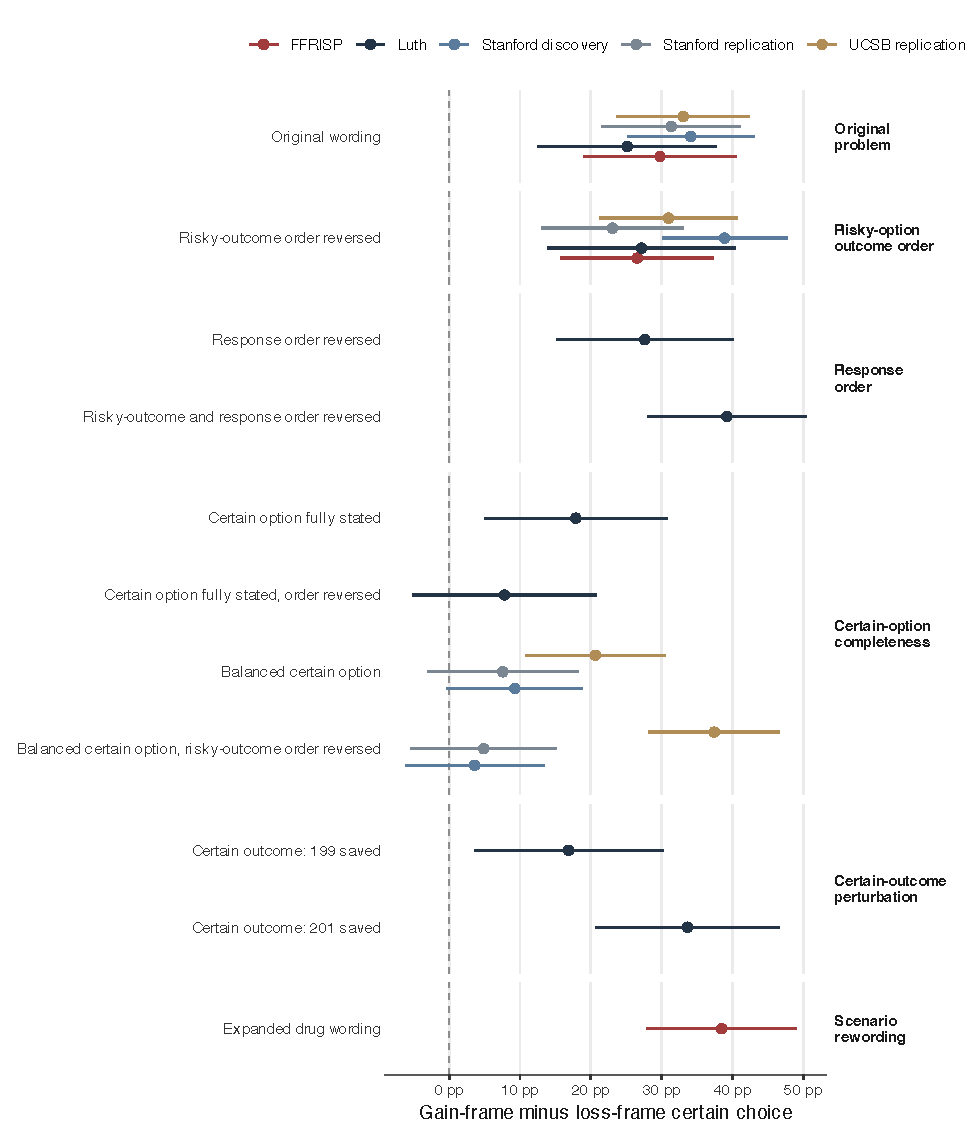
\includegraphics[width=\textwidth]{../figs/family_effects.pdf}
  \caption{Gain-frame minus loss-frame differences in choosing the certain option, organized by manipulation family. Points are differences in percentage points; lines are 95 percent confidence intervals based on HC2 standard errors. Every point is a within-survey estimate; the three 2018 studies appear separately. The defective Luth natural-frequency pair is omitted.}
  \label{fig:family-effects}
\end{figure}
\FloatBarrier

\subsection{The original problem}

The original wording reproduced the classic directional contrast in every survey that fielded it. In FFRISP, \FFROriginalGain\ percent chose the certain option in the gain frame and \FFROriginalLoss\ percent did so in the loss frame. The difference was \FFROriginalEffect\ percentage points, with a 95 percent confidence interval from \FFROriginalLow\ to \FFROriginalHigh\ ($N=\FFROriginalN$). In Luth, the corresponding proportions were \LuthOriginalGain\ and \LuthOriginalLoss\ percent, a difference of \LuthOriginalEffect\ points with an interval from \LuthOriginalLow\ to \LuthOriginalHigh\ ($N=\LuthOriginalN$). In the three 2018 experiments, the original-format contrasts ranged from \ProtzkoOriginalMin\ to \ProtzkoOriginalMax\ points. The original problem therefore establishes the benchmark against which every manipulation below is read: a framing contrast between roughly \LuthOriginalEffect\ and \ProtzkoOriginalMax\ points in five samples recruited nine years apart.

\subsection{Reordering outcomes within the risky option}

If the framing contrast depended on which risky outcome respondents read first, stating the failure outcome before the success outcome would change it. It did not. The contrast was \FFRArmRiskyFlipEffect\ points in FFRISP and \LuthArmRiskyFlipEffect\ points in Luth under the reversed order, close to each survey's original-wording estimate, and between \ProtzkoFlipMin\ and \ProtzkoFlipMax\ points in the flipped cells of the three 2018 experiments. This manipulation was fielded in all five surveys, so its effect on the contrast can be estimated five times, each as a within-survey change against that survey's original wording: the pooled change is \FlipChangeEffect\ points (95 percent CI \FlipChangeLow\ to \FlipChangeHigh; \FlipChangeK\ surveys; Appendix Table~\ref{tab:manipulation-meta}). The 2018 factorial interaction agrees ($\ProtzkoFlipInteraction$ points, $p=\ProtzkoFlipP$). The order of outcomes inside the risky option is not load-bearing for the effect.

\subsection{Reordering the response options}

Listing the risky option first, rather than the certain option, likewise left the contrast intact: \LuthArmResponseOrderEffect\ points in the Luth response-order pair, and \LuthArmRiskyResponseEffect\ points when the response-order reversal was combined with the risky-outcome reversal. Neither estimate is reliably different from the Luth original. Where the options appear on the screen, like the order of clauses inside them, does not carry the effect.

\subsection{Stating the certain option completely}

The certain option in the original problem describes only one outcome: 200 saved, or 400 dead, with the complement left unstated. Completing the description is the one manipulation in this archive that reliably changed the size of the contrast. In Luth, fully stating the certain option cut the contrast to \LuthArmBalancedEffect\ points, and additionally reversing the order of its two components cut it to \LuthArmBalancedReversedEffect\ points, the smallest valid estimate in the archive. The 2018 experiments randomized a functionally described balanced certain option: their balanced-cell contrasts ranged from \ProtzkoBalancedMin\ to \ProtzkoBalancedMax\ points across the three studies, against \ProtzkoOriginalMin\ to \ProtzkoOriginalMax\ points in their original-format cells. Fully stating the certain option was fielded in four surveys, and its within-survey change against the original wording is negative in all four: pooled, it reduced the framing contrast by \BalancedAttenuation\ points (95 percent CI \BalancedAttenuationLow\ to \BalancedAttenuationHigh; \BalancedChangeK\ surveys; Appendix Table~\ref{tab:manipulation-meta}). Combining balancing with the risky-outcome flip reduced the contrast by a pooled \BalancedFlipAttenuation\ points across the three 2018 studies, but that synthesis is imprecise (95 percent CI $\BalancedFlipAttenuationLow$ to \BalancedFlipAttenuationHigh) because the UCSB estimate for the combined cell runs the other way. The respondent-level 2018 factorial model agrees: balancing reduced the contrast by \ProtzkoExplicitAttenuation\ points (95 percent CI \ProtzkoExplicitAttenuationLow\ to \ProtzkoExplicitAttenuationHigh, $p\ProtzkoExplicitP$), with a three-way interaction of \ProtzkoThreeWay\ points ($p=\ProtzkoThreeWayP$). Every balanced-cell contrast nevertheless remains positive (Table~\ref{tab:family-effects}; Appendix Table~\ref{tab:protzko-effects} reports the pooled design cells). Completing the certain option attenuates the effect; it does not eliminate it.

\subsection{Moving the sure outcome: 199, 200, and 201}

Two Luth pairs changed the certain outcome to 199 saved and 401 lost, or to 201 saved and 399 lost. Within each pair the gain and loss descriptions remain extensionally equivalent, so each pair is a local test of description invariance while the sure outcome moves one life below or above the gamble's expected outcome. The contrast was \LuthArmLowerEffect\ points at 199 and \LuthArmUpperEffect\ points at 201, positive at both values. Figure~\ref{fig:invariance-profile} shows the frame-specific choice rates at all three values: the gain and loss profiles remain separated across the range. Because the between-frame comparison is randomized at each value, the one-life shift does not confound it. But three nearby binary-choice points provide only a local choice profile; they cannot identify a value function, locate frame-specific certainty equivalents, or distinguish prospect theory from linguistic and representational accounts.

\begin{figure}[tbp]
  \centering
  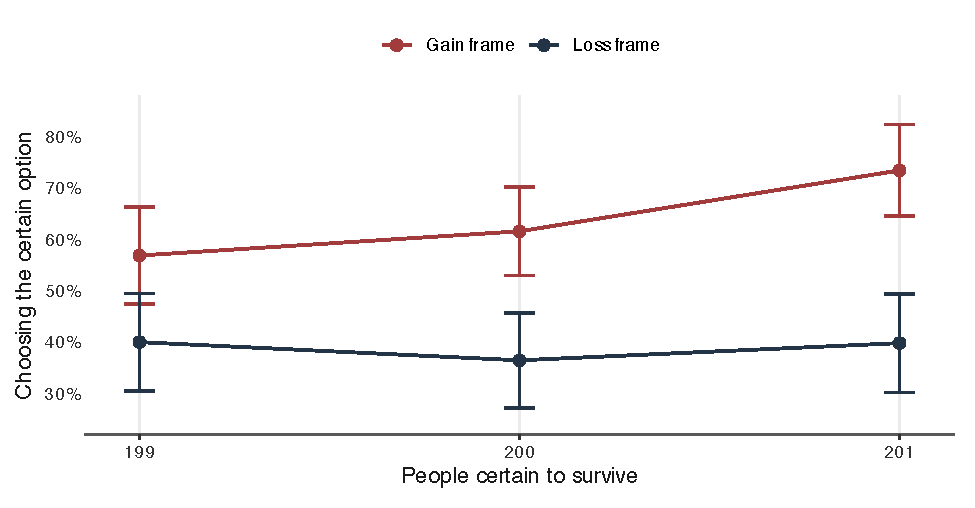
\includegraphics[width=\textwidth]{../figs/invariance_profile.pdf}
  \caption{Local description-invariance profile in the Luth primary sample. Points are percentages choosing the certain option at each sure number of survivors; lines connect the three observed values within each frame. Vertical lines are 95 percent confidence intervals for each cell mean. At every value, the gain and loss descriptions specify the same objective sure outcome and the same risky option. Description invariance therefore predicts overlapping gain- and loss-frame profiles.}
  \label{fig:invariance-profile}
\end{figure}

\subsection{Rewording the scenario}

The expanded FFRISP variant rewrote the task wholesale: a drug-choice scenario with the probabilities expressed as chances, added contextual detail, and no reference to an Asian disease. The contrast was \FFRArmRewordingEffect\ points, the largest FFRISP estimate. The effect does not depend on the canonical text. The ninth planned Luth pair, which expressed the risky probabilities as natural frequencies, would have spoken to the same question, but its deployed loss-frame stem named different programs than its response options, so both of its arms are excluded.

\subsection{Within-survey heterogeneity and archive-wide synthesis}

Joint tests summarize the wording variation within each 2009 survey. The three FFRISP estimates range from \FFRMinimumEffect\ to \FFRMaximumEffect\ points, and a joint test does not reject equality across the three wordings, $F=\FFRHeterogeneityF$, $p=\FFRHeterogeneityP$. The Luth estimates range from \LuthMinimumEffect\ to \LuthMaximumEffect\ points, and its joint test rejects a common framing contrast, $F=\LuthHeterogeneityF$, $p=\LuthHeterogeneityP$.

Across all \ArchiveMetaK\ independent contrasts and \ArchiveMetaN\ analyzed choices, the random-effects mean was \ArchiveMetaEffect\ percentage points (95 percent CI \ArchiveMetaLow\ to \ArchiveMetaHigh). Heterogeneity was substantial ($I^2=\ArchiveMetaISquared\%$), and the 95 percent prediction interval ranged from \ArchiveMetaPredLow\ to \ArchiveMetaPredHigh\ points. The interval remains positive but is much wider than the confidence interval for the mean. It therefore supports a stable average direction while rejecting the idea that one effect magnitude characterizes every archived task. The manipulation-effect synthesis in Appendix Table~\ref{tab:manipulation-meta} organizes that heterogeneity: because each manipulation is differenced against its own survey's original wording, those within-survey changes attribute the variation to description features rather than to samples, and the certain-option completeness manipulations account for the large attenuations. Appendix Figure~\ref{fig:archive-meta} displays all constituent estimates.

\begin{table}[H]
\centering
\caption{\label{tab:archive-meta}Archive-wide synthesis of gain-loss framing contrasts}
\centering
\begin{threeparttable}
\begin{tabular}[t]{lrr}
\toprule
Model & Mean difference [95\% CI] & 95\% prediction interval\\
\midrule
Random effects & 24.7 [19.7, 29.7] & 2.7 to 46.6\\
Fixed effect sensitivity & 25.2 [23.0, 27.4] & --\\
\bottomrule
\end{tabular}
\begin{tablenotes}[para]
\item Note: Entries are gain-frame minus loss-frame percentage points across 23 independent randomized contrasts. The primary model uses REML and Knapp--Hartung inference. This synthesis describes the recovered archive and is not a literature-wide meta-analysis.
\end{tablenotes}
\end{threeparttable}
\end{table}


\subsection{Post-choice explanations}

The Luth open-ended responses provide a limited check on how respondents described their choices. Among \OpenEndedN\ respondents with a valid primary code, the two most common categories were a chance that everyone survives and certainty or risk aversion. Those categories were similarly common in the gain and loss frames: the chance category appeared for \OpenEndedChanceGain\ percent and \OpenEndedChanceLoss\ percent of respondents, respectively, and the certainty category for \OpenEndedCertaintyGain\ and \OpenEndedCertaintyLoss\ percent. The adjusted loss-minus-gain differences were \OpenEndedChanceDiff\ and \OpenEndedCertaintyDiff\ percentage points, and none of the eight category differences survived Holm adjustment (Appendix Table~\ref{tab:open-ended-frame-effects}). Thus, the coded explanations do not supply parallel evidence that framing shifted these broad, post-choice rationales. Because the explanations followed choice and the historical coding scheme has overlapping categories, they cannot identify the process that produced the choice difference.

\subsection{Sensitivity}

The original-wording estimates are stable to the two planned sample sensitivities. Survey weighting changes the FFRISP point estimate modestly but leaves a clear positive contrast. Including all completed Luth respondents produces nearly the same estimate as the screened analysis. Table~\ref{tab:sensitivity} reports both checks.

\subsection{Moderation by education}

Table~\ref{tab:education-meta} reports the education-by-frame interaction estimated separately within each of the five experiments, each adjusting for its own randomized wording or design factors, and the random-effects synthesis of the five coefficients. Every experiment's point estimate is positive, though each is individually imprecise. The synthesis estimates that the framing contrast grows by \EducationMetaEffect\ points per education category (95\% CI \EducationMetaLow\ to \EducationMetaHigh), with essentially no between-experiment heterogeneity ($I^2=\EducationMetaISquared\%$). The respondent-level pooled models agree: \ModeratorArchiveInteraction\ points per category across the three 2018 experiments and \ModeratorAllInteraction\ points across all five experiments (95\% CI \ModeratorAllLow\ to \ModeratorAllHigh). The individual experiments are imprecise, so the synthesis, not any single survey, carries the estimate. These results do not support a claim that greater measured knowledge eliminates the framing contrast; if anything, the contrast is larger at higher education. They are exploratory, may reflect residual differences in sample composition or measurement, and are not tests of intelligence; education is an imperfect proxy for reasoning ability, and the political-knowledge interaction in Appendix Table~\ref{tab:moderators} is imprecise and does not survive Holm adjustment.

\begin{table}[H]
\centering
\caption{\label{tab:education-meta}Education moderation of the framing contrast, by experiment}
\centering
\begin{threeparttable}
\begin{tabular}[t]{lrr}
\toprule
Experiment & N & Interaction [95\% CI]\\
\midrule
FFRISP probability panel & 887 & 5.7 [-1.1, 12.5]\\
Luth volunteer panel & 1,568 & 3.5 [-2.8, 9.8]\\
Stanford discovery & 1,645 & 3.2 [-1.6, 8.1]\\
Stanford replication & 1,440 & 4.6 [-0.3, 9.5]\\
UCSB replication & 1,500 & 3.2 [-2.9, 9.2]\\
\midrule
Random-effects synthesis & 7,040 & 4.0 [2.7, 5.2]\\
\bottomrule
\end{tabular}
\begin{tablenotes}[para]
\item Note: Entries are the change in the gain-minus-loss framing contrast, in percentage points, per one-category increase in education, from linear probability models with HC2 standard errors that adjust for each experiment's randomized wording or design factors. The synthesis row pools the five interaction coefficients with a REML random-effects model and Knapp--Hartung inference. Education is an imperfect proxy for reasoning ability, and all rows are exploratory.
\end{tablenotes}
\end{threeparttable}
\end{table}


\section{Discussion}

The experiments yield a simple result with an important qualification. Gain versus loss language moved risky choice in the classic direction in every valid archived contrast. The original-wording contrast survived survey weighting in the probability panel and inclusion of attention-check failures in the volunteer panel. Fully stating or balancing the certain option attenuated the contrast in every survey that fielded that manipulation, while reversing the risky option's outcome order did not reliably change it in any of the five surveys. At the same time, the effect's magnitude varies considerably, and the archive-wide synthesis is inconsistent with one common effect size.

The probability-panel result expands the range of people for whom the classic directional effect has been observed. Later comparisons across online panels have also found the Asian Disease effect in samples that differ in composition and recruitment \parencite{chandler2019panels,stagnaro2026samples}. Such evidence supports generality of direction more directly than exact generality of magnitude. The weighted FFRISP estimate is smaller than its unweighted estimate, and the two panels should not be treated as interchangeable representations of the U.S. adult population.

The wording results fit a literature in which apparently redundant details alter the representation of the options. Fully stating or explicitly balancing an option reduces the contrast in some formulations, yet does not remove it. Reversing probability, response order, or internal order also does not mechanically erase the effect, consistent with an experiment that found neither order manipulation significant \parencite{peng2017mixed}. These patterns agree with evidence that description valence and completeness explain part, but not all, of risky-choice framing \parencite{dekay2024mismatched,dekay2026complete}. They are less compatible with treating one canonical wording as a context-free measure of a fixed individual bias.

The 199 and 201 pairs sharpen the invariance result: the gain-loss gap is positive at all three sure outcomes even though each pair remains extensionally equivalent. As the results section emphasizes, three nearby binary-choice points provide only a local choice profile; they cannot identify a value function, locate frame-specific certainty equivalents, or distinguish prospect theory from linguistic and representational accounts.

The exploratory moderator results also narrow the old manuscript's claims. Education is an imperfect proxy for reasoning ability, and political knowledge is a domain-specific factual measure. Neither justifies the label intelligence. Prior work has reported relations with reflection and numeracy \parencite{stanovich1998individual,leboeuf2003deep,peters2008numeracy}, but two experiments using several cognitive-style measures found no reliable predictor of frame-consistent choice beyond the frame itself \parencite{mandel2018cognitive}. The current intervals allow both small and meaningful moderation, so stronger conclusions require a design with validated cognitive measures and planned power for treatment heterogeneity.

Several limitations remain. The analysis plan is retrospective. Luth is an opt-in sample, and the attention screen changes its target population. One planned wording pair is unusable because of a deployment error. The 2018 questionnaire, sampling documentation, original scripts, and November 2019 manuscript remain missing; consequently, we can verify the recorded factorial assignments and outcomes but not every historical procedural or reporting claim. Moderator data are missing for some respondents and were collected in separate panel surveys. The instruments were not designed to adjudicate modern formal accounts of description valence or gist. The archived explanations were elicited after choice rather than with a process-tracing design, unlike work that manipulates or records the order of reasons \parencite{wall2020query,composto2025query}. Their coding also has unresolved category overlap and no documented adjudication rule. It cannot establish respondents' decision processes or distinguish psychological from moral-reason accounts \parencite{zuradzki2026reasons}. Finally, the original ethics protocol numbers and current data-sharing authorization are not present in the archive and must be verified before journal submission.

The most defensible conclusion is therefore bounded. Risky-choice framing was directionally robust across the five archived experiments, but its measured size was not a property of gain and loss labels alone. Small choices about what to state, what to leave implicit, and where to place information can materially change the estimate.

\section*{Data and code availability}

The public repository contains the deidentified respondent-level analysis files for all five experiments, the complete analysis code, source manifests with checksums, recode and join ledgers, tests, and generated exhibits. The released files are minimized at construction: they carry only the columns the analysis consumes, replace the FFRISP design codes with anonymized ranks, and use deterministic sequential case identifiers that reproduce from the sources without linking to any panel identifier. Raw survey and panel exports contain IP addresses, respondent or panel identifiers, ZIP codes, user-agent strings, and open text, so they remain in a restricted source directory; the published manifests allow an authorized copy to be verified by checksum, and the pipeline reruns all analyses from the released files when the raw exports are absent. The open-ended response text is likewise restricted; only aggregate coding-reliability results are released.

\printbibliography

\clearpage
\appendix
\setcounter{table}{0}
\renewcommand{\thetable}{SI\arabic{table}}
\renewcommand{\theHtable}{SI\arabic{table}}
\section{Fieldwork and sample construction}

\subsection{FFRISP recruitment and retention}

The archived final methodology report identifies Abt SRBI as the organization responsible for sampling, recruitment, panel maintenance, respondent support, and most survey administration \parencite{ackermann2009ffrisp}. The weighting section reports 3,723 sampled addresses, whereas the fieldwork disposition section reports 3,184 worked cases. The surviving records do not reconcile those denominators, so we do not calculate a recruitment response rate from them. The report does establish that 1,145 eligible adults were selected, 1,000 enrolled, and 902 completed the final monthly survey.

Monthly invitations began by email. Abt SRBI followed nonrespondents by email and telephone for up to two weeks, then by post. Table~\ref{tab:ffrisp-retention} shows the resulting wave counts.

\begin{table}[H]
\centering
\caption{\label{tab:ffrisp-retention}FFRISP monthly survey retention}
\centering
\begin{threeparttable}
\begin{tabular}[t]{rllrr}
\toprule
Wave & Month & Host & Completes & Percent of 1,000\\
\midrule
1 & Oct 2008 & Knowledge Networks & 989 & 98.9\%\\
2 & Nov 2008 & Knowledge Networks & 978 & 97.8\%\\
3 & Dec 2008 & Knowledge Networks & 979 & 97.9\%\\
4 & Jan 2009 & Abt SRBI & 974 & 97.4\%\\
5 & Feb 2009 & Abt SRBI & 970 & 97.0\%\\
6 & Mar 2009 & Abt SRBI & 963 & 96.3\%\\
7 & Apr 2009 & Abt SRBI & 955 & 95.5\%\\
8 & May 2009 & Knowledge Networks & 950 & 95.0\%\\
9 & Jun 2009 & Knowledge Networks & 934 & 93.4\%\\
10 & Jul 2009 & Abt SRBI & 929 & 92.9\%\\
11 & Aug 2009 & Abt SRBI & 913 & 91.3\%\\
12 & Sep 2009 & Stanford & 902 & 90.2\%\\
\bottomrule
\end{tabular}
\begin{tablenotes}[para]
\item Note: Source is Table 1 of the archived FFRISP Final Methodology Report. Percentages retain one decimal place here; the report rounded them to whole percentages.
\end{tablenotes}
\end{threeparttable}
\end{table}


\subsection{Analysis flow and condition allocation}

Tables~\ref{tab:sample-flow} and \ref{tab:condition-counts} show every analytical restriction and the number of completed and analyzed respondents in each frame. The six missing Luth outcomes among attention-check passers occur in the defective pair, so outcome missingness does not further reduce the valid-pair primary sample.

\begin{table}[H]
\centering
\caption{\label{tab:sample-flow}Analysis sample flow}
\centering
\begin{threeparttable}
\begin{tabular}[t]{>{\raggedright\arraybackslash}p{3.2cm}>{\raggedright\arraybackslash}p{6.6cm}>{\raggedleft\arraybackslash}p{1.2cm}}
\toprule
Sample & Stage & N\\
\midrule
FFRISP & Source export (starting N) & 902\\
FFRISP & After valid panel-ID restriction & 898\\
FFRISP & Final analytic sample (nonmissing outcome) & 887\\
Luth & Source export (starting N) & 2,330\\
Luth & After attention-check restriction & 2,017\\
Luth & After valid-instrument restriction & 1,777\\
Luth & Final analytic sample (nonmissing outcome) & 1,777\\
Luth & Sensitivity: all completed, valid outcome & 2,048\\
Stanford discovery & Source export (starting N) & 1,647\\
Stanford discovery & Final analytic sample (nonmissing first choice) & 1,645\\
Stanford replication & Source export (starting N) & 1,442\\
Stanford replication & Final analytic sample (nonmissing first choice) & 1,440\\
UCSB replication & Source export (starting N) & 1,500\\
UCSB replication & Final analytic sample (nonmissing choice) & 1,500\\
\bottomrule
\end{tabular}
\begin{tablenotes}[para]
\item Note: FFRISP's numeric-identifier step removes four test or nonpanel records. The Luth valid-pair step removes the defective natural-frequency pair. The final rows identify the primary analytic sample for each survey. The Luth sensitivity row retains completed respondents with a valid outcome without the attention screen. The 2018 rows show source-to-analysis attrition separately for each of the three study exports.
\end{tablenotes}
\end{threeparttable}
\end{table}


\begin{table}[H]
\centering
\caption{\label{tab:condition-counts}Completed and analyzed respondents by wording pair and design cell}
\centering
\fontsize{8}{10}\selectfont
\begin{threeparttable}
\begin{tabular}[t]{llrrrr}
\toprule
\multicolumn{2}{c}{ } & \multicolumn{2}{c}{Completed} & \multicolumn{2}{c}{Analyzed} \\
\cmidrule(l{3pt}r{3pt}){3-4} \cmidrule(l{3pt}r{3pt}){5-6}
Sample & Wording & Gain & Loss & Gain & Loss\\
\midrule
FFRISP & Original wording & 141 & 162 & 141 & 158\\
FFRISP & Risky-outcome order reversed & 165 & 131 & 163 & 129\\
FFRISP & Expanded drug wording & 151 & 148 & 149 & 147\\
Luth & Original wording & 138 & 121 & 125 & 107\\
Luth & Certain outcome: 199 saved & 125 & 120 & 109 & 105\\
Luth & Certain outcome: 201 saved & 111 & 123 & 98 & 103\\
Luth & Natural-frequency wording & 147 & 133 & Excluded & Excluded\\
Luth & Response order reversed & 137 & 121 & 119 & 109\\
Luth & Certain option fully stated & 122 & 138 & 107 & 119\\
Luth & Certain option fully stated, order reversed & 130 & 136 & 115 & 115\\
Luth & Risky-outcome order reversed & 127 & 119 & 108 & 97\\
Luth & Risky-outcome and response order reversed & 147 & 135 & 128 & 113\\
Stanford discovery & Original wording & 212 & 216 & 212 & 216\\
Stanford discovery & Risky-outcome order reversed & 213 & 201 & 213 & 200\\
Stanford discovery & Balanced certain option & 195 & 208 & 195 & 208\\
Stanford discovery & Balanced certain option, risky-outcome order reversed & 210 & 192 & 210 & 191\\
Stanford replication & Original wording & 179 & 182 & 179 & 182\\
Stanford replication & Risky-outcome order reversed & 200 & 172 & 200 & 171\\
Stanford replication & Balanced certain option & 173 & 169 & 173 & 169\\
Stanford replication & Balanced certain option, risky-outcome order reversed & 183 & 184 & 182 & 184\\
UCSB replication & Original wording & 186 & 192 & 186 & 192\\
UCSB replication & Risky-outcome order reversed & 186 & 185 & 186 & 185\\
UCSB replication & Balanced certain option & 184 & 193 & 184 & 193\\
UCSB replication & Balanced certain option, risky-outcome order reversed & 187 & 187 & 187 & 187\\
\bottomrule
\end{tabular}
\begin{tablenotes}[para]
\item Note: Completed counts use the canonical exports after removal of four FFRISP test or nonpanel records. Analyzed counts require a nonmissing outcome and, for Luth, passage of the pretreatment attention check. The 2018 rows show all four factorial cells within each study export. Dashes mark the excluded pair whose deployed stem and response labels named different programs.
\end{tablenotes}
\end{threeparttable}
\end{table}


\subsection{Per-survey estimates}

Table~\ref{tab:effects} reports the same 2009 framing contrasts as Table~\ref{tab:family-effects}, grouped by survey rather than by manipulation.

\begin{table}[H]
\centering
\caption{\label{tab:effects}2009 experiments: certain choice by frame and wording}
\centering
\begin{threeparttable}
\begin{tabular}[t]{lrrr}
\toprule
Wording & Gain frame & Loss frame & Difference [95\% CI]\\
\midrule
\addlinespace[0.3em]
\multicolumn{4}{l}{\textbf{FFRISP probability panel}}\\
\hspace{1em}Original wording & 70.9\% & 41.1\% & 29.8 [19.0, 40.6]\\
\hspace{1em}Risky-outcome order reversed & 52.1\% & 25.6\% & 26.6 [15.7, 37.4]\\
\hspace{1em}Expanded drug wording & 70.5\% & 32.0\% & 38.5 [27.9, 49.1]\\
\addlinespace[0.3em]
\multicolumn{4}{l}{\textbf{Luth volunteer panel}}\\
\hspace{1em}Original wording & 61.6\% & 36.4\% & 25.2 [12.5, 37.8]\\
\hspace{1em}Certain outcome: 199 saved & 56.9\% & 40.0\% & 16.9 [3.5, 30.2]\\
\hspace{1em}Certain outcome: 201 saved & 73.5\% & 39.8\% & 33.7 [20.6, 46.7]\\
\hspace{1em}Response order reversed & 58.8\% & 31.2\% & 27.6 [15.1, 40.2]\\
\hspace{1em}Certain option fully stated & 60.7\% & 42.9\% & 17.9 [4.9, 30.9]\\
\hspace{1em}Certain option fully stated, order reversed & 56.5\% & 48.7\% & 7.8 [-5.2, 20.8]\\
\hspace{1em}Risky-outcome order reversed & 60.2\% & 33.0\% & 27.2 [13.9, 40.5]\\
\hspace{1em}Risky-outcome and response order reversed & 57.8\% & 18.6\% & 39.2 [28.0, 50.5]\\
\bottomrule
\end{tabular}
\begin{tablenotes}[para]
\item Note: Entries in the middle columns are percentages choosing the certain option. Differences are gain-frame minus loss-frame percentage points. Confidence intervals use HC2 standard errors. The defective Luth natural-frequency pair is omitted.
\end{tablenotes}
\end{threeparttable}
\end{table}


\subsection{Deployed and reconstructed treatment text}

Table~\ref{tab:wording-inventory} crosswalks every deployed gain-loss pair and 2018 design cell using the same condition labels as the results exhibits. The scenario stem is the standard 600-person disease problem unless the table identifies the expanded drug scenario. ``Success outcome first'' means that the risky option states the one-third all-survive outcome before the two-thirds none-survive outcome; ``failure outcome first'' reverses those clauses. This inventory preserves distinctions that the compact results table necessarily suppresses.

Table~\ref{tab:verbatim-wording} reports the treatment text itself, graded by its evidentiary status. The FFRISP rows quote the archived deployed item text verbatim. The Luth rows are reconstructed from the archived draft descriptions and checked against the deployed questionnaire PDFs; the deployed September questionnaire, not the corrected November revision, is the record of what respondents saw. The 2018 rows are functional descriptions from the recorded factor coding, corroborated for every respondent by the Qualtrics block-assignment labels in the Stanford exports, because the fielded text is unavailable.

\begin{landscape}
\begingroup
\setlength{\tabcolsep}{3.5pt}
\begingroup\fontsize{8}{10}\selectfont

\begin{longtable}[t]{>{\raggedright\arraybackslash}p{1.3cm}>{\raggedright\arraybackslash}p{3.2cm}>{\raggedright\arraybackslash}p{3.6cm}>{\raggedright\arraybackslash}p{3.6cm}>{\raggedright\arraybackslash}p{6.4cm}>{\raggedright\arraybackslash}p{1.5cm}}
\caption{\label{tab:wording-inventory}Deployed wording-pair and design-cell inventory}\\
\toprule
Sample & Wording & Certain option: gain & Certain option: loss & Other deployed feature & Status\\
\midrule
\endfirsthead
\caption[]{Deployed wording-pair and design-cell inventory \textit{(continued)}}\\
\toprule
Sample & Wording & Certain option: gain & Certain option: loss & Other deployed feature & Status\\
\midrule
\endhead

\endfoot
\bottomrule
\endlastfoot
FFRISP & Original wording & 200 people will be saved & 400 people will die & Success outcome first; certain option first & Analyzed\\
FFRISP & Risky-outcome order reversed & 200 people will be saved & 400 people will die & Failure outcome first; certain option first & Analyzed\\
FFRISP & Expanded drug wording & 100\% chance of preventing 200 deaths & 100\% chance the disease kills 400 & Expanded stem; success outcome first; certain option first & Analyzed\\
Luth & Original wording & 200 people will be saved & 400 people will die & Success outcome first; certain option first & Analyzed\\
Luth & Certain outcome: 199 saved & 199 people will be saved & 401 people will die & Success outcome first; certain option first & Analyzed\\
Luth & Certain outcome: 201 saved & 201 people will be saved & 399 people will die & Success outcome first; certain option first & Analyzed\\
Luth & Natural-frequency wording & 200 people will be saved & 400 people will die & Uses '1 in 3' and '2 in 3'; deployed loss stem names Programs C and D while response options name Programs A and B & Excluded\\
Luth & Response order reversed & 200 people will be saved & 400 people will die & Success outcome first; risky option first & Analyzed\\
Luth & Certain option fully stated & 200 saved; 400 not saved & 400 die; 200 not die & Success outcome first; certain option first & Analyzed\\
Luth & Certain option fully stated, order reversed & 400 not saved; 200 saved & 200 not die; 400 die & Success outcome first; certain option first & Analyzed\\
Luth & Risky-outcome order reversed & 200 people will be saved & 400 people will die & Failure outcome first; certain option first & Analyzed\\
Luth & Risky-outcome and response order reversed & 200 people will be saved & 400 people will die & Failure outcome first; risky option first & Analyzed\\
2018 factorial & Original wording & Certain option stated one outcome & Certain option stated one outcome & Original internal order & Analyzed\\
2018 factorial & Risky-outcome order reversed & Certain option stated one outcome & Certain option stated one outcome & Failure outcome first & Analyzed\\
2018 factorial & Balanced certain option & Certain option stated both outcomes & Certain option stated both outcomes & Original internal order & Analyzed\\
2018 factorial & Balanced certain option, risky-outcome order reversed & Certain option stated both outcomes & Certain option stated both outcomes & Failure outcome first & Analyzed\\*
\end{longtable}
\endgroup{}

\endgroup

\begingroup
\setlength{\tabcolsep}{3.5pt}
\begingroup\fontsize{8}{10}\selectfont

\begin{longtable}[t]{>{\raggedright\arraybackslash}p{1.2cm}>{\raggedright\arraybackslash}p{2.6cm}>{\raggedright\arraybackslash}p{1.7cm}>{\raggedright\arraybackslash}p{6.2cm}>{\raggedright\arraybackslash}p{6.2cm}>{\raggedright\arraybackslash}p{2.6cm}}
\caption{\label{tab:verbatim-wording}Deployed and reconstructed treatment text}\\
\toprule
Sample & Wording & Record & Gain-frame options & Loss-frame options & Stem\\
\midrule
\endfirsthead
\caption[]{Deployed and reconstructed treatment text \textit{(continued)}}\\
\toprule
Sample & Wording & Record & Gain-frame options & Loss-frame options & Stem\\
\midrule
\endhead

\endfoot
\bottomrule
\multicolumn{6}{@{}p{21.0cm}@{}}{\rule{0pt}{1em}Note: Option texts separate the certain and risky options with ||. Verbatim rows quote the archived deployed item text; reconstructed rows quote the archived draft descriptions checked against the deployed questionnaire PDFs; functional rows describe the 2018 cells from the recorded factor coding and Qualtrics block labels because the fielded text is unavailable.}\\
\endlastfoot
FFRISP & Original wording & verbatim & If Program A is adopted, 200 people will be saved. || If Program B is adopted, there is 1/3 probability that 600 people will be saved, and 2/3 probability that no people will be saved. & If Program A is adopted 400 people will die. || If Program B is adopted there is 1/3 probability that nobody will die, and 2/3 probability that 600 people will die. & Standard 600-person disease stem\\
\addlinespace
FFRISP & Risky-outcome order reversed & verbatim & If Program A is adopted, 200 people will be saved. || If Program B is adopted, there is a 2/3 probability that no people will be saved, and 1/3 probability that 600 people will be saved. & If Program A is adopted 400 people will die. || If Program B is adopted there is a 2/3 probability that 600 people will die and 1/3 probability that nobody will die. & Standard 600-person disease stem\\
\addlinespace
FFRISP & Expanded drug wording & verbatim & If Drug A is offered to everyone, there is a 100\% chance that it will prevent the deaths of 200 of the people. || If Drug B is offered to everyone, there is: a 1/3 chance that it will prevent the deaths of all 600 people and a 2/3 chance that it will not prevent the deaths of any of the 600 people. & If Drug A is offered to everyone, there is a 100\% chance that the disease will kill 400 people. || If Drug B is offered to everyone, there is: a 1/3 chance that the disease will not kill anyone and a 2/3 chance that the disease will kill all 600 people. & Expanded drug-scenario stem\\
\addlinespace
Luth & Original wording & reconstructed & If Program A is adopted, 200 people will be saved. || If Program B is adopted, there is a 1/3 probability that 600 people will be saved, and a 2/3 probability that no people will be saved. & If Program A is adopted, 400 people will die. || If Program B is adopted, there is a 1/3 probability that nobody will die, and a 2/3 probability that 600 people will die. & Standard 600-person disease stem\\
\addlinespace
Luth & Certain outcome: 199 saved & reconstructed & As the original wording, with 200 changed to 199 in the certain option. & As the original wording, with 400 changed to 401 in the certain option. & Standard 600-person disease stem\\
\addlinespace
Luth & Certain outcome: 201 saved & reconstructed & As the original wording, with 200 changed to 201 in the certain option. & As the original wording, with 400 changed to 399 in the certain option. & Standard 600-person disease stem\\
\addlinespace
Luth & Natural-frequency wording & reconstructed & If Program A is adopted, 200 people will be saved. || If Program B is adopted, there is a 1 in 3 chance that all 600 people will be saved, and a 2 in 3 chance that no people will be saved. & Deployed loss-frame stem named Programs C and D while the response options named Programs A and B; the archived draft's loss-frame quotation repeats the gain-frame text, so the deployed loss text is not reliably reconstructable. & Standard 600-person disease stem\\
\addlinespace
Luth & Response order reversed & reconstructed & As the original wording, with the risky option listed first and the certain option second. & As the original wording, with the risky option listed first and the certain option second. & Standard 600-person disease stem\\
\addlinespace
Luth & Certain option fully stated & reconstructed & 200 people will be saved, and 400 people will not be saved. || Risky option as the original wording. & 400 people will die, and 200 people will not die. || Risky option as the original wording. & Standard 600-person disease stem\\
\addlinespace
Luth & Certain option fully stated, order reversed & reconstructed & If Program A is adopted, 400 people will not be saved, and 200 people will be saved. || Risky option as the original wording. & If Program A is adopted, 200 people will not die, and 400 people will die. || Risky option as the original wording. & Standard 600-person disease stem\\
\addlinespace
Luth & Risky-outcome order reversed & reconstructed & If Program B is adopted, there is a 2/3 probability that no people will be saved, and a 1/3 probability that 600 people will be saved. || Certain option as the original wording. & If Program B is adopted, there is a 2/3 probability that 600 people will die and a 1/3 probability that nobody will die. || Certain option as the original wording. & Standard 600-person disease stem\\
\addlinespace
Luth & Risky-outcome and response order reversed & reconstructed & Risky option listed first with its outcome order reversed; certain option as the original wording. The archived draft's frame attribution for its quotations is internally inconsistent, so only the structure is reconstructed. & Risky option listed first with its outcome order reversed; certain option as the original wording. The archived draft's frame attribution for its quotations is internally inconsistent, so only the structure is reconstructed. & Standard 600-person disease stem\\
\addlinespace
2018 factorial & Original wording & functional & Certain option states the saved outcome only; risky option in original outcome order. & Certain option states the deaths outcome only; risky option in original outcome order. & Fielded text unavailable; block labels name the arm 'original wording'\\
\addlinespace
2018 factorial & Risky-outcome order reversed & functional & Certain option states the saved outcome only; risky option with outcome order reversed. & Certain option states the deaths outcome only; risky option with outcome order reversed. & Fielded text unavailable; block labels name the arm 'internal flip'\\
\addlinespace
2018 factorial & Balanced certain option & functional & Certain option states both the saved and the not-saved outcomes; risky option in original outcome order. & Certain option states both the deaths and the not-die outcomes; risky option in original outcome order. & Fielded text unavailable; block labels name the arm 'explicit balancing'\\
\addlinespace
2018 factorial & Balanced certain option, risky-outcome order reversed & functional & Certain option states both outcomes; risky option with outcome order reversed. & Certain option states both outcomes; risky option with outcome order reversed. & Fielded text unavailable; block labels name the arm 'explicit balancing plus internal flip'\\*
\end{longtable}
\endgroup{}

\endgroup
\end{landscape}

\clearpage
\section{Weighting, sensitivity, and exploratory moderation}

FFRISP base weights adjusted for unequal household selection probabilities, screener nonresponse, within-household adult selection, panel nonenrollment, and population coverage. The report documents calibration to 2007 American Community Survey margins for tenure, children, household size, age, gender, Hispanic ethnicity, race, and education. It also documents trimming and raking for wave 1. The archived weight file contains variables for all 12 waves, including the month 12 weight used below, but the archive contains no corresponding month 12 production memo.

\begin{table}[H]
\centering
\caption{\label{tab:sensitivity}Original-wording sensitivity analyses}
\centering
\begin{threeparttable}
\begin{tabular}[t]{lrr}
\toprule
Specification & N & Difference [95\% CI]\\
\midrule
FFRISP original wording, unweighted & 299 & 29.8 [19.0, 40.6]\\
FFRISP original wording, survey weighted & 299 & 24.9 [10.7, 39.1]\\
Luth original wording, attention check passed & 232 & 25.2 [12.5, 37.8]\\
Luth original wording, all completed respondents & 259 & 24.5 [12.6, 36.4]\\
\bottomrule
\end{tabular}
\begin{tablenotes}[para]
\item Note: Differences are gain-frame minus loss-frame percentage points for the original wording. The weighted FFRISP interval uses its stratified, clustered survey design; other intervals use HC2 standard errors.
\end{tablenotes}
\end{threeparttable}
\end{table}


\begin{table}[H]
\centering
\caption{\label{tab:moderators}Exploratory moderator interactions}
\centering
\fontsize{8}{10}\selectfont
\begin{threeparttable}
\begin{tabular}[t]{llrrrr}
\toprule
Measure & Unit & N & Interaction [95\% CI] & p & Holm p\\
\midrule
FFRISP education & one-category increase & 887 & 5.7 [-1.1, 12.5] & 0.099 & 0.210\\
Luth education & one-category increase & 1568 & 3.5 [-2.8, 9.8] & 0.276 & 0.276\\
Luth political knowledge & zero-to-one increase & 1579 & 18.7 [-1.5, 38.9] & 0.070 & 0.210\\
Three 2018 experiments pooled, education & one-category increase & 4585 & 3.8 [0.8, 6.8] & 0.012 & 0.049\\
All five experiments, education & one-category increase & 7040 & 4.0 [1.5, 6.6] & 0.002 & 0.008\\
\bottomrule
\end{tabular}
\begin{tablenotes}[para]
\item Note: Positive interactions indicate a larger gain-minus-loss contrast at higher moderator values. Models include wording indicators and all wording-by-frame interactions. Political knowledge is a five-item factual battery, not an intelligence measure. These analyses are exploratory.
\end{tablenotes}
\end{threeparttable}
\end{table}


\clearpage
\section{2018 factorial experiments and archive-wide synthesis}

\subsection{Source reconstruction}

Table~\ref{tab:sample-flow} reports the source-to-analysis flow for all three 2018 study exports. The received anonymous file orders the Stanford replication first, the Stanford discovery second, and the UCSB replication third. Its first 4,589 rows otherwise match that source-derived stack except at combined row 3,089, corresponding to Stanford discovery row 1,647: the source first choice is missing, whereas the combined value is zero. Row 4,590 is entirely blank. The source-first pipeline preserves the missing response and omits the blank row; the detailed discrepancy remains documented in the repository's source-flow artifact.

\subsection{Study-specific and pooled framing contrasts}

Figure~\ref{fig:protzko-effects} shows the twelve gain-minus-loss differences across the three 2018 experiments, and Table~\ref{tab:protzko-effects} reports the four design cells after pooling the three studies with study indicators. Every estimate is positive. Balanced-certain-option estimates are generally smaller, although the UCSB balanced cell with the internal flip is an exception; the pooled factorial interaction therefore summarizes an average change rather than a deterministic rule for every study and design cell.

\begin{table}[H]
\centering
\caption{\label{tab:protzko-effects}2018 Stanford/UCSB factorial experiments: certain choice by framing condition}
\centering
\begin{threeparttable}
\begin{tabular}[t]{llrrr}
\toprule
Certain option & Internal order & Gain frame & Loss frame & Difference [95\% CI]\\
\midrule
Unbalanced & Original internal order & 70.4\% & 37.5\% & 32.9 [27.5, 38.3]\\
Unbalanced & Internal flip & 63.9\% & 32.7\% & 31.3 [25.8, 36.8]\\
Balanced & Original internal order & 57.6\% & 45.1\% & 12.6 [6.8, 18.4]\\
Balanced & Internal flip & 52.3\% & 37.2\% & 15.1 [9.4, 20.8]\\
\bottomrule
\end{tabular}
\begin{tablenotes}[para]
\item Note: The three source exports contribute 4,585 respondents with valid first choices. Differences are gain-frame minus loss-frame percentage points from linear probability models with study indicators and HC2 standard errors. Cell percentages are unadjusted. In balanced conditions, the certain option stated both outcomes.
\end{tablenotes}
\end{threeparttable}
\end{table}


\begin{figure}[H]
  \centering
  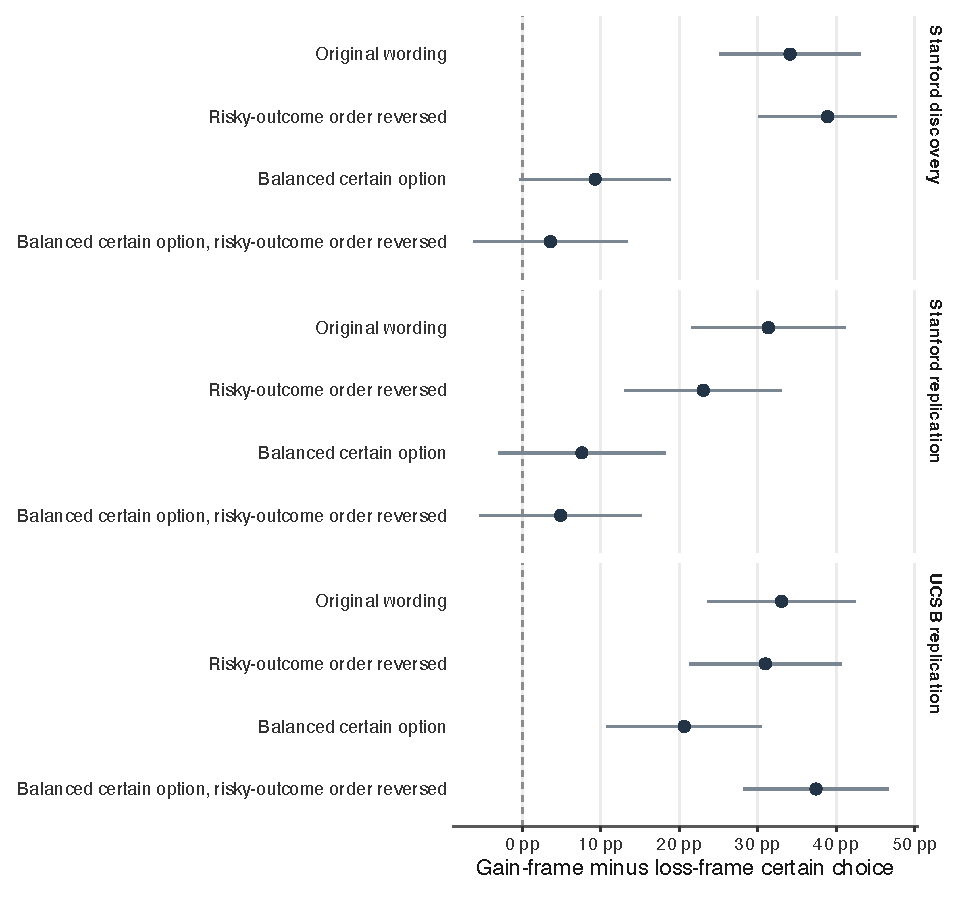
\includegraphics[width=0.92\textwidth]{../figs/protzko_frame_effects.pdf}
  \caption{Study-specific framing contrasts in the archived 2018 experiments. Points are gain-frame minus loss-frame differences in percentage points; horizontal lines are 95 percent confidence intervals based on HC2 standard errors. Each respondent contributes only the first recorded framing choice.}
  \label{fig:protzko-effects}
\end{figure}

\subsection{Manipulation-effect synthesis}

Table~\ref{tab:manipulation-meta} reports, for every deployed manipulation, the change in the framing contrast relative to the same survey's original wording. Manipulations fielded in several surveys are pooled with a random-effects model; single-survey manipulations report the one available within-survey difference. The reversal of the risky option's outcome order, fielded in all five surveys, does not change the contrast; the certain-option completeness manipulations reduce it in every survey that fielded them, with the UCSB balanced-plus-flip cell as the one exception.

\begin{table}[H]
\centering
\caption{\label{tab:manipulation-meta}Manipulation effects on the framing contrast, synthesized across surveys}
\centering
\begin{threeparttable}
\begin{tabular}[t]{lrr}
\toprule
Manipulation & Surveys & Change [95\% CI]\\
\midrule
Risky-outcome order reversed & 5 & -1.3 [-7.8, 5.3]\\
Response order reversed & 1 & 2.5 [-15.2, 20.2]\\
Risky-outcome and response order reversed & 1 & 14.1 [-2.7, 30.9]\\
Certain option fully stated (balanced) & 4 & -18.1 [-31.2, -5.0]\\
Certain option fully stated, order reversed & 1 & -17.3 [-35.3, 0.7]\\
Balanced certain option, risky-outcome order reversed & 3 & -17.5 [-65.0, 30.1]\\
Certain outcome: 199 saved & 1 & -8.3 [-26.5, 10.0]\\
Certain outcome: 201 saved & 1 & 8.5 [-9.5, 26.5]\\
Expanded drug wording & 1 & 8.7 [-6.4, 23.8]\\
\bottomrule
\end{tabular}
\begin{tablenotes}[para]
\item Note: Each entry is the change in the gain-minus-loss framing contrast, in percentage points, relative to the same survey's original wording; both arms are randomized within the survey. Rows with several surveys pool the within-survey changes with a REML random-effects model and Knapp--Hartung inference; single-survey rows report the one available difference with a normal interval. Changes from the same survey share that survey's original-wording arm, so rows are not independent of one another; within each row, surveys are independent.
\end{tablenotes}
\end{threeparttable}
\end{table}


\subsection{Archive-wide forest plot}

Figure~\ref{fig:archive-meta} displays every independent contrast in the separate synthesis module. The red vertical line is the random-effects mean and the shaded band is its 95 percent confidence interval. The band describes uncertainty about the average; the wider prediction interval reported in Table~\ref{tab:archive-meta} describes expected between-contrast variation.

\begin{figure}[H]
  \centering
  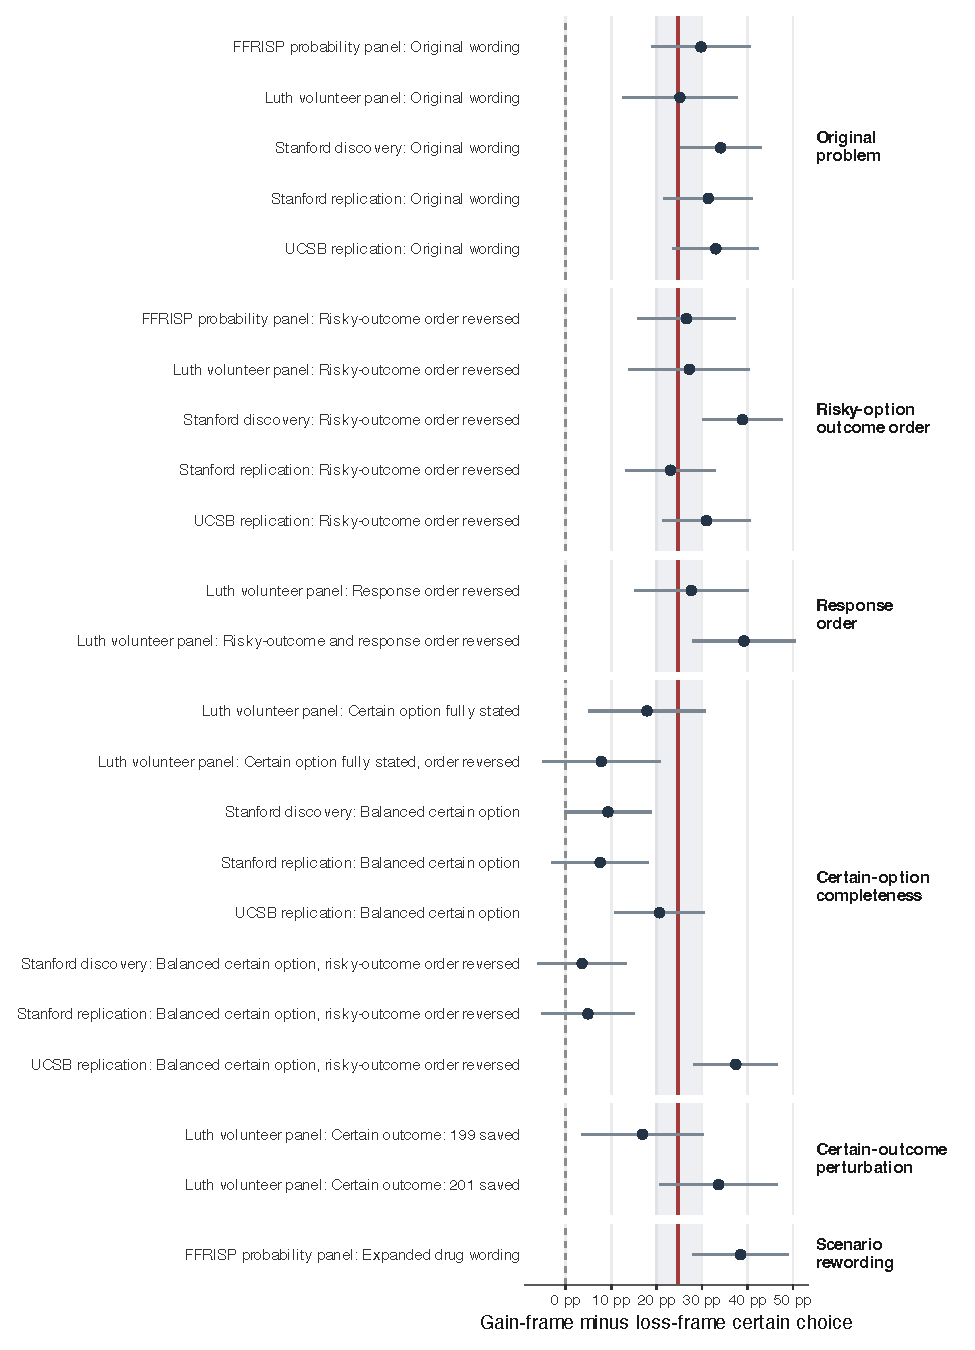
\includegraphics[width=0.82\textwidth]{../meta/figures/archive_meta_forest.pdf}
  \caption{Archive-wide forest plot, grouped by manipulation family. Points are gain-frame minus loss-frame differences in choosing the certain option; horizontal lines are 95 percent confidence intervals. The red line and shaded band show the REML random-effects mean and its 95 percent confidence interval. The synthesis covers the available archive, not the published literature.}
  \label{fig:archive-meta}
\end{figure}

\clearpage
\section{Audit of the open-ended coding}

The Luth instrument asked respondents to explain their choices. A later coding project assigned up to two of eight categories: no stated reason; equal expected value; certainty or risk aversion; a chance that everyone survives; saving more people; ease of understanding; other; or a claim that one option was better without a reason. The workbook contains 2,330 substantive rows and one blank trailing row. Anne and Jeremy both supplied valid primary codes for 2,295 responses.

We audit the independent codes and do not use the workbook's reconciled ``True Score.'' The archive does not document a reproducible adjudication algorithm. A contemporaneous memo also notes overlap among certainty, chance, and number-saved categories; ambiguity between no reason and other; and inconsistent use of the better-choice category. Table~\ref{tab:open-ended-reliability} reports overall agreement. Table~\ref{tab:open-ended-categories} shows that reliability varies across categories, especially for rare or overlapping codes. No open-ended response text is reproduced or exported by the pipeline.

\begin{table}[H]
\centering
\caption{\label{tab:open-ended-reliability}Reliability of the archived open-ended coding}
\centering
\fontsize{9}{11}\selectfont
\begin{threeparttable}
\begin{tabular}[t]{lrrr}
\toprule
Measure & N & Agreement & Cohen's kappa\\
\midrule
Primary-code exact agreement & 2,295 & 78.8\% & 0.731\\
Full code-set exact agreement & 2,295 & 72.3\% & --\\
At least one assigned code overlaps & 2,295 & 81.4\% & --\\
\bottomrule
\end{tabular}
\begin{tablenotes}[para]
\item Note: Anne and Jeremy supplied the two code sets. Primary-code statistics use responses with valid primary codes from both coders. Each coder could add a secondary category. Dashes mark set-based measures without a single multicategory Cohen's kappa in this audit.
\end{tablenotes}
\end{threeparttable}
\end{table}


\begin{table}[H]
\centering
\caption{\label{tab:open-ended-categories}Category-specific reliability of primary open-ended codes}
\centering
\fontsize{9}{11}\selectfont
\begin{threeparttable}
\begin{tabular}[t]{rlrrr}
\toprule
Code & Category & Anne n & Jeremy n & Binary kappa\\
\midrule
1 & No stated reason & 169 & 170 & 0.882\\
2 & Equal expected value & 162 & 142 & 0.824\\
3 & Certainty or risk aversion & 582 & 636 & 0.786\\
4 & Risk offers chance all survive & 726 & 718 & 0.760\\
5 & Saves more people & 443 & 349 & 0.638\\
6 & Easier to understand & 12 & 6 & 0.331\\
7 & Other & 137 & 163 & 0.508\\
8 & Better choice without a reason & 64 & 111 & 0.603\\
\bottomrule
\end{tabular}
\begin{tablenotes}[para]
\item Note: Counts and binary kappa values use primary codes only. The instructions allowed multiple categories. A contemporaneous memo identifies overlap among codes 3, 4, and 5 and ambiguity involving codes 1, 7, and 8.
\end{tablenotes}
\end{threeparttable}
\end{table}


These codes describe how two coders classified post-choice explanations. We use the primary codes descriptively to ask whether the distribution of stated reasons differs between gain and loss frames, adjusting for wording pair. The frame comparisons are not a second outcome and do not establish a psychological mechanism; respondents' explanations may be retrospective rationalizations. The results show whether the explanations add information about how respondents represented the options, while preserving the coding audit's uncertainty.

\begin{table}[H]
\centering
\caption{\label{tab:open-ended-frame-effects}Framing differences in coded post-choice explanations}
\centering
\fontsize{8}{10}\selectfont
\begin{threeparttable}
\begin{tabular}[t]{lrrrrrr}
\toprule
Category & N & Gain \% & Loss \% & Loss - gain [95\% CI] & p & Holm p\\
\midrule
No stated reason & 1752 & 8.0 & 6.9 & -1.1 [-3.5, 1.4] & 0.390 & 1.000\\
Equal expected value & 1752 & 7.0 & 6.6 & -0.4 [-2.8, 2.0] & 0.738 & 1.000\\
Certainty or risk aversion & 1752 & 23.7 & 26.7 & 2.8 [-1.3, 6.9] & 0.177 & 1.000\\
Risk offers chance all survive & 1752 & 33.3 & 31.1 & -2.0 [-6.4, 2.3] & 0.361 & 1.000\\
Saves more people & 1752 & 18.6 & 19.4 & 0.9 [-2.8, 4.6] & 0.639 & 1.000\\
Easier to understand & 1752 & 0.2 & 0.8 & 0.6 [-0.1, 1.3] & 0.086 & 0.684\\
Other & 1752 & 6.0 & 5.5 & -0.5 [-2.7, 1.7] & 0.665 & 1.000\\
Better choice without a reason & 1752 & 3.1 & 2.9 & -0.3 [-1.9, 1.3] & 0.733 & 1.000\\
\bottomrule
\end{tabular}
\begin{tablenotes}[para]
\item Note: Percentages use Anne's primary code among attention-check passers with a valid instrument and framing outcome. Models adjust for wording pair and use HC2 standard errors. Codes classify explanations after the choice; they are descriptive and do not identify a causal mechanism.
\end{tablenotes}
\end{threeparttable}
\end{table}


The most common coded explanations were a chance that everyone survives, certainty or risk aversion, and saving more people. Their frame differences were small relative to their uncertainty, and no category survives Holm adjustment. The open-ended material therefore complements the choice results by documenting respondents' stated representations without turning retrospective explanations into evidence for a single mechanism.

\end{document}
